%&pdflatex
\documentclass[12pt]{article}
\usepackage[margin=1.0in]{geometry}

\usepackage{g-util}
\usepackage{caratula.met}
\usepackage{amsfonts, amsmath, amssymb, amsthm}
\usepackage{graphicx, float, hyperref, wrapfig}
\graphicspath{ {./plots/} }
%\usepackage[xetex]{xcolor}

% \theoremstyle{plain}
\newtheorem{prop}{Proposición}
\newtheorem{lema}{Lema}
% \theoremstyle{remark}
\newtheorem{obs}{Observación}
% \theoremstyle{definition}
\newtheorem{defi}{Definición}

\setcounter{MaxMatrixCols}{12}
\newcommand{\Gpmatrix}[1]{\ensuremath{\begin{pmatrix} #1 \end{pmatrix}}}
\newcommand{\Gbmatrix}[1]{\ensuremath{\begin{bmatrix} #1 \end{bmatrix}}}
\newcommand{\sub}[3]{\ensuremath{#1_{#2,#3}}}
\newcommand{\supra}[2]{\ensuremath{#1^#2}}

\renewcommand{\figurename}{Fig.}
\renewcommand{\listfigurename}{Figuras}
\renewcommand{\contentsname}{Secciones}
\renewcommand{\refname}{Bibliografía}

\begin{document}

\titulo{TP1 - Trabajamos y nos divertimos...}
%\subititulo{}

\fecha{\today}

\materia{Métodos Numéricos}
\grupo{Grupo 8}

\integrante{Cappella Lewi, F. Galileo}{653/20}{galileocapp@gmail.com}
\integrante{Anachure, Juan Pablo}{99/16}{janachure@gmail.com}

\maketitle
\tableofcontents

\pagebreak
\section{Introducción}
\label{sec:intro}

\begin{wrapfigure}{l}{0.35\textwidth}
	\centering
	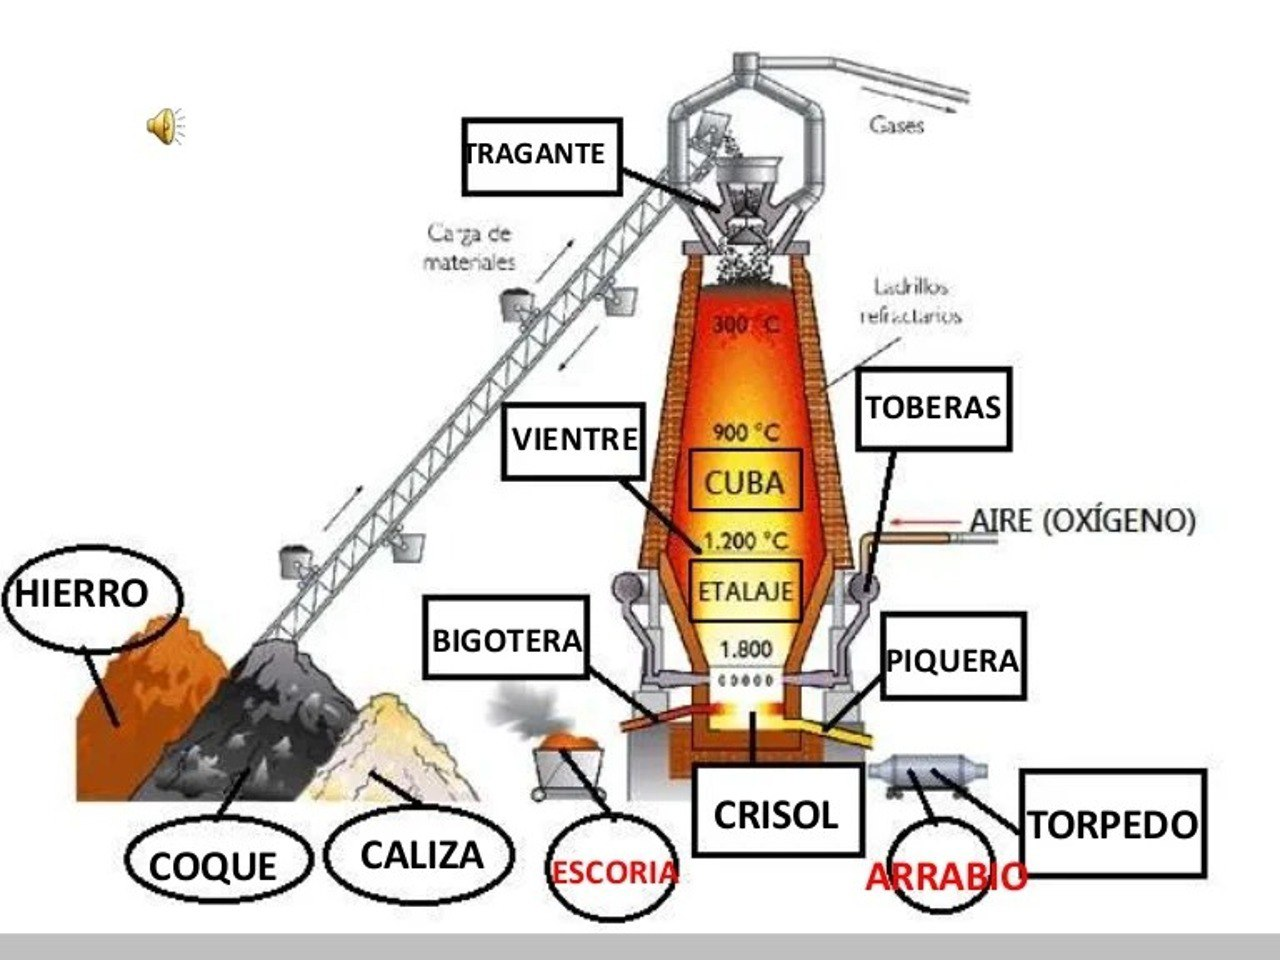
\includegraphics[width=0.35\textwidth]{alto_horno}
	\caption{Diarama de las partes de un alto horno}
	\label{fig:alto_horno}
\end{wrapfigure}

\paragraph{} Los altos hornos son un tipo de horno metalúrgico, usados para producir metales industriales. Están formados por una pared circular usualmente de acero y ladrillos refractarios, lo que permite fundir distintos metales dentro. En la Figura \ref{fig:furnace} se puede ver un diagrama de la sección horizontal de un horno.
\paragraph{} Estos hornos suelen trabajar con temperaturas internas de 900ºC a 1300ºC \cite{how.it.works}, y en las paredes externas se suelen medir temperaturas de entre 50ºC y 200ºC. Dentro de la pared es importante la posición de la isoterma de 500ºC, ya que si esta se encuentra cerca del exterior (ver Sección \ref{sec:peligrosidad}) la integridad del horno podría estar en riesgo.
\paragraph{} En este trabajo se estudia una manera de calcular las temperaturas dentro de la pared, buscando poder estimar la posición de la isoterma. Para ello se utiliza una discretización de la ecuación del calor de Laplace (Sección \ref{sec:modelado}). 

\begin{figure}[H]
	\centering
	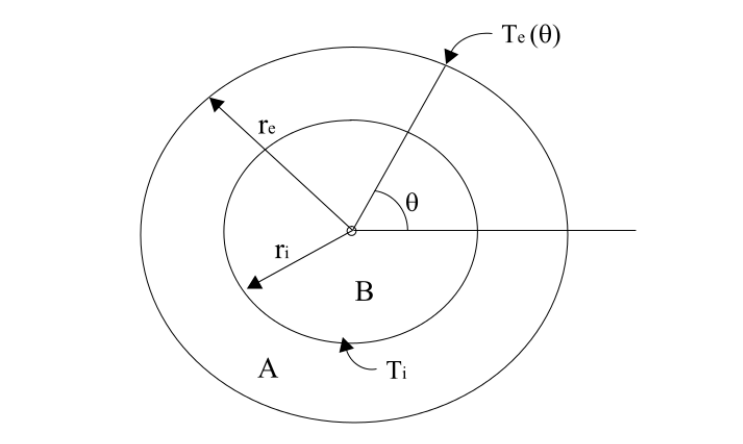
\includegraphics[scale=0.55]{alto_discreto}
	\caption{Sección horizontal de un horno}
	\label{fig:furnace}
\end{figure}

\paragraph{} El problema de encontrar la isoterma, y medición de peligrosidad se puede resolver utilizando un modelo que requiere de un conjunto de temperaturas medidas en diferentes ángulos. Esto es procesado utilizando un sistema de ecuaciones lineales, por lo que será de interés utilizar métodos que permitan encontrar soluciones a este tipo de sistemas, particularmente este trabajo esta orientado en la utilización de Eliminación Gaussiana y factorización LU. Finalmente, utilizando los resultados de dichos métodos se quiere evaluar la peligrosidad del horno.

\section{Desarrollo}

\subsection{Modelado}
\label{sec:modelado}

\paragraph{} La ecuación del calor Laplace afirma que en estado estacionario cualquier temperatura \(T(r, \theta)\), dada por la posición dentro de la pared del horno en coordenadas polares \((r, \theta)\) que representan al radio y el ángulo polar, cumple la siguiente ecuación: 

\begin{equation}
\label{eq:laplace}
  0 = \frac{\partial^2T(r,\ \theta)}{\partial r^2} + \frac{1}{r} \frac{\partial^2T(r,\ \theta)}{\partial r} + \frac{1}{r^2} \frac{\partial^2T(r,\ \theta)}{\partial\theta^2}
\end{equation}

\paragraph{} Para poder utilizarla para resolver el problema computacionalmente, discretizamos el dominio a coordenadas polares. Tomando una partición \(0 = \theta_0 < \theta_1 < ... < \theta_n = 2\pi\) en \(n\) ángulos discretos con \(\theta_k - \theta_{k-1} = \Delta\theta\) para \(k = 1, ..., n\) y una partición \(r_i = r_0 < r_1 < ... < r_m = r_e\) en \(m+1\) radios discretos con \(r_j - r_{j-1} = \Delta r\) para \(j = 1, ..., m\). Tomamos \(\sub{t}{j}{k} = T(r_j, \theta_k)\) y transformamos a la ecuación (\ref{eq:laplace}) en un conjunto de ecuaciones lineales sobre las incógnitas \(\sub{t}{j}{k}\), aproximando así a \(T\) por la siguiente fórmula de diferencias finitas: %TODO: Too similar to the assignment

\begin{equation}
\label{eq:laplace.finita}
0 = \frac{\sub{t}{j-1}{k} - 2\sub{t}{j}{k} + \sub{t}{j+1}{k}}{(\Delta r)^2} + \frac{\sub{t}{j}{k} - \sub{t}{j-1}{k}}{r \Delta r} + \frac{\sub{t}{j}{k-1} - 2\sub{t}{j}{k} + \sub{t}{j}{k+1}}{r^2 (\Delta \Theta)^2}
\end{equation}

Que podemos reescribir como una combinación lineal de cinco temperaturas:
\begin{equation}
\label{eq:laplace.split}
0 = \sub{t}{j-1}{k} (\frac{1}{(\Delta r)^{2}} + \frac{-1}{r \Delta r}) + \sub{t}{j}{k} (\frac{-2}{(\Delta r)^2} + \frac{1}{r \Delta r} + \frac{-2}{(r \Delta \Theta)^{2}}) + \sub{t}{j+1}{k} \frac{1}{(\Delta r)^{2}} + \sub{t}{j}{k-1} \frac{1}{(r \Delta \Theta)^{2}} + \sub{t}{j}{k+1} \frac{1}{(r\Delta \Theta)^{2}}
\end{equation}
%Aunque para simplificar la notación vamos a nombrar cada coeficiente, por lo que nos queda: \\ %TODO: Renombrar coeficientes para que tengan más sentido
%\begin{equation}
%\label{eq:laplace.split}
%0 = \alpha_r\sub{t}{j-1}{k} + \beta_r\sub{t}{j}{k} + \gamma_r\sub{t}{j+1}{k} + \chi_r\sub{t}{j}{k-1} + \chi_r\sub{t}{j}{k+1}
%\end{equation}
%\(
%\tab \alpha_r = \frac{1}{(\Delta r)^{2}} + \frac{-1}{r \Delta r} \\
%\tab \beta_r = \frac{-2}{(\Delta r)^2} + \frac{1}{r \Delta r} + \frac{-2}{(r \Delta \Theta)^{2}} \\
%\tab \gamma_r = \frac{1}{(\Delta r)^{2}} \\ 
%\tab \chi_r = \frac{1}{(r \Delta \Theta)^{2}}
%\)
\paragraph{} Ahora armamos un sistema de ecuaciones para cada \(\sub{t}{j}{k}\), que podemos representar matricialmente de la forma \(At = b\). Donde \(A \in \mathbb{R}^{(m+1)n \times (m+1)n}\) es una matriz con las primeras y últimas \(n\) filas iguales a la identidad (por las temperaturas externas e internas, que son datos), y el resto corresponde a una instancia de la ecuación (\ref{eq:laplace.split}); \(t \in \mathbb{R}^{(m+1)n}\) es el vector de incógntias con los radios "estirados" uno arriba del otro; Y  \(b \in \mathbb{R}^{(m+1)n}\) es el vector de resultados que tiene las temperaturas internas en los primeros \(n\) valores, las externas en los últimos \(n\) valores, y el resto todos ceros. \\
%Se ve descripto cómo construir la matriz con la siguiente función:  %TODO: Es horrible
%\begin{equation}
%\sub{a}{i}{j} = \begin{cases}
  %\alpa & \text{if } n < i \leq mn \land  \\
  %\beta & \text{if } i = j \\
  %\gamma & \text{if } \\
  %\chi & \text{if } \\
  %1 & \text{if } i \leq n \lor mn < i \land j = i\\
  %0 & \text{otherwise} \\
%\end{cases} \forall 1 \leq i, j \leq (m+1)n
%\end{equation}
En la ecuación (\ref{eq:example}) mostramos un ejemplo de cómo queda el sistema con \(r_i = 1,\ r_e = 3,\ mp1 = 3,\ n = 3,\ \sub{t}{i}{1} = \sub{t}{i}{2} = \sub{t}{i}{3} = 1500,\ \sub{t}{e}{1} = \sub{t}{e}{2} = \sub{t}{e}{3} = 150\).

\begin{equation}
\label{eq:example}
\Gpmatrix{
  1 & 0 & 0 & 0 & 0 & 0 & 0 & 0 & 0 \\
  0 & 1 & 0 & 0 & 0 & 0 & 0 & 0 & 0 \\
  0 & 0 & 1 & 0 & 0 & 0 & 0 & 0 & 0 \\
  \frac{1}{2} & 0 & 0 & -\frac{2}{\pi^2} - \frac{3}{2} & \frac{1}{\pi^2} & \frac{1}{\pi^2} & 1 & 0 & 0 \\
  0 & \frac{1}{2} & 0 & \frac{1}{\pi^2} & -\frac{2}{\pi^2} - \frac{3}{2} & \frac{1}{\pi^2} & 0 & 1 & 0 \\
  0 & 0 & \frac{1}{2} & \frac{1}{\pi^2} & \frac{1}{\pi^2} & -\frac{2}{\pi^2} - \frac{3}{2} & 0 & 0 & 1 \\
  0 & 0 & 0 & 0 & 0 & 0 & 1 & 0 & 0 \\
  0 & 0 & 0 & 0 & 0 & 0 & 0 & 1 & 0 \\
  0 & 0 & 0 & 0 & 0 & 0 & 0 & 0 & 1 \\
} \cdot \Gpmatrix{
  \sub{t}{1}{1} \\
  \sub{t}{1}{2} \\
  \sub{t}{1}{3} \\
  \sub{t}{2}{1} \\
  \sub{t}{2}{2} \\
  \sub{t}{2}{3} \\
  \sub{t}{3}{1} \\
  \sub{t}{3}{2} \\
  \sub{t}{3}{3} \\
} = \Gpmatrix{
  1500 \\
  1500 \\
  1500 \\
  0 \\
  0 \\
  0 \\
  150 \\
  150 \\
  150 \\
}
\end{equation}

Demostramos en el apéndice \ref{appendix:justificacion} que se puede aplicar la Eliminación Gaussiana sin pivotear filas.

\subsection{Implementación}

\paragraph{} Implementamos este sistema en \texttt{C++}. Primero programamos matrices usando vectores de la \texttt{STL}. Luego implementamos funciones que resuelvan sistemas de ecuaciones usando Eliminación Gaussiana o factorización LU. Y finalmente recibimos los datos y guardamos los resultados en archivos pasados por parámetros. \\
También armamos una herramienta en \texttt{Python} para correr el programa y analizar los resultados, armando los gráficos vistos a través de este informe (como la Figura \ref{fig:temperature}). \\
Todo el código se puede ver adjuntado al informe, junto con explicaciones de cómo usarlo. \\

\begin{figure}[H]
\centering
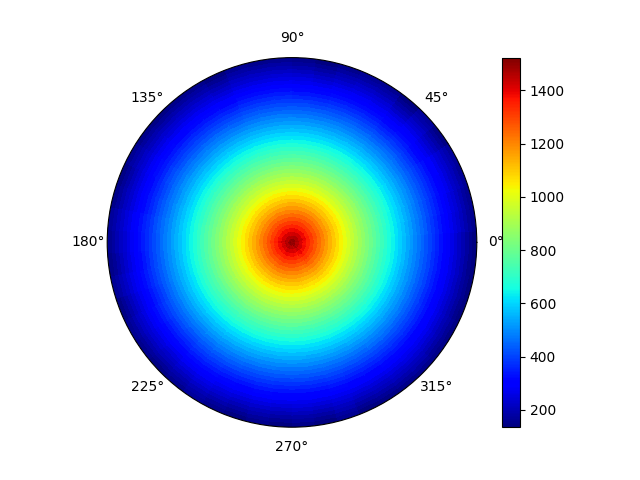
\includegraphics[scale=0.5]{complete.0.temperature}
\caption{Temperatura calculada dentro del horno}
\label{fig:temperature}
\end{figure}

%\subsubsection{Optimización Matriz "en banda"}

%\paragraph{} Por cómo construimos la matriz, luego aplicar la eliminación Gaussiana, nos queda una matriz "en banda", lo que en este caso significa que en todas las filas sólo tiene máximo \(n+1\) elementos diferentes a cero. \\
%Por lo que podemos aprovechar y sólo operar sobre esos valores, reduciendo tanto la memoria usada por el programa, como la cantidad de operaciones hechas para resolver el sistema. \\
%En la figura \ref{fig:memory.band.nband} se puede apreciar el espacio ahorrado por esta optimización. \\
%Y en la figura \ref{fig:times.band.nband} se nota que esta optimización no mejoró mucho el tiempo de operación. Esto se debe a que el órden del sistema no dejó de ser \(\bigO{((m+1)n)^3}\). %TODO: Calcular bien el orden
%%TODO: Figuras memory.band.nband y times.band.nband

%\begin{figure}[H] %TODO: Fig.banda
%\centering
%\includegraphics[scale=0.5]{times.band.nband.100.1}
%\caption{Comparación del tiempo para resolver una instancia del sistema entre banda y no banda}
%\label{fig:gauss.banda}
%\end{figure}

\section{Estimando la isoterma}
\label{sec:peligrosidad}

\paragraph{} En la sección \ref{sec:intro} planteamos que la razón principal de querer resolver este problema es querer calcular la posición de la isoterma de 500ºC, ya que si está "muy cerca" (ver sección \ref{sec:peligrosidad.distance}) la estructura del horno estaría en riesgo.

\begin{figure}[H]
\centering
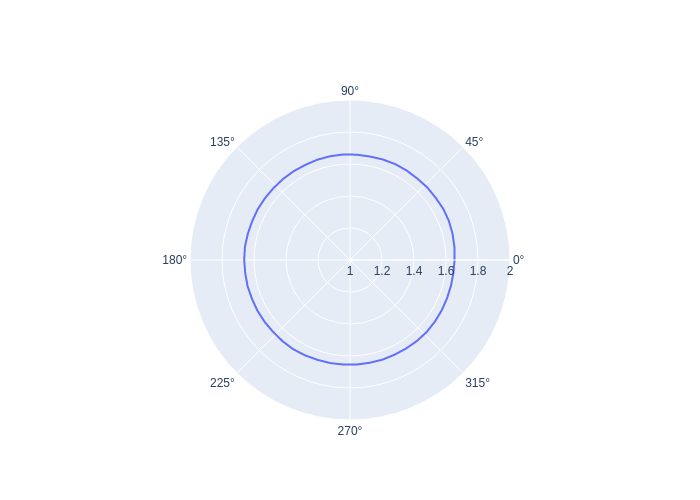
\includegraphics[scale=0.5]{complete.0.isotherm}
\caption{Posición estimada de la isoterma}
\label{fig:isotherm.pos}
\end{figure}

\paragraph{} Para encontrarla buscamos dos puntos dentro de un mismo ángulo que "rodeen" la temperatura buscada, y luego aproximamos linealmente la posición donde se encuentra entre estos dos puntos. 

\subsection{Midiendo la Peligrosidad}
\label{sec:peligrosidad.distance}

\paragraph{} Una vez encontrada la isoterma, es importante decidir si el horno está en un estado peligroso o seguro. \\
Pero habría que conocer más sobre cómo está armado un alto horno para poder sacar conclusiones sobre qué tan peligrosa es la posición de la isoterma. Aunque preliminarmente se puede ver (Figura \ref{fig:isotherm_by_inner}) que si el "punto de ruptura" se encuentra antes del 75\% de la pared hay poco margen de error, ya que hasta ese punto la isoterma se mueve rápido hacia el exterior.

\section{Experimentación} 

%\subsection{Consutrucción de las instancias}
%Para experimentar se construyen instancias para cada experimento. En el experimento 1 se definio un $\epsilon = 10^{-4}}$. Para el experimento 2, se realiza una serie de variaciones a la temperatura externa en los siguientes valores [v1,v2,v3,v4] y se evalua donde se encuentra la isoterma buscada. Para el experimento 3, en las instancias construidas se deje estatico a la cantidad de angulos que tendra el horno mientras se varia la cantidad de radios que puede tener el horno. Finalmente en el experimento 4 intercambiamos la variable estatica del experimento 3 para que evaluar el impacto del cambio de radios en las soluciones.  %TODO: Epsilon en función del número de condición %TODO: Una explicación de cómo armamos y variamos las entradas por cada experimento

\subsection{Resultados esperados}
\label{sec:expected}

\paragraph{} La cátedra nos proveyó con una serie de tests, con su input y un output esperado. Al correr nuestro programa con este input nos encontramos con que los resultados conseguidos no eran iguales a los esperados (ver figura \ref{fig:expected.diffs}). \\
Para confirmar si este error es aceptable usamos el número de condición, que es un número calculado a partir de la matriz que nos permite definir un rango de error alrededor del resultado esperado, dentro del cual, si se encuentran nuestros resultados, es aceptable y común por errores de redondeo (ver sección \ref{sec:rounding}).

\paragraph{} Se puede notar que el error crece hacia el centro del horno. Esto se debe a que el algoritmo implementado para resolver el sistema despeja las temperaturas más internas en función de las más externas, por lo que los errores cometidos se van acumulando desde afuera hacia adentro.

\begin{figure}[H]
\centering
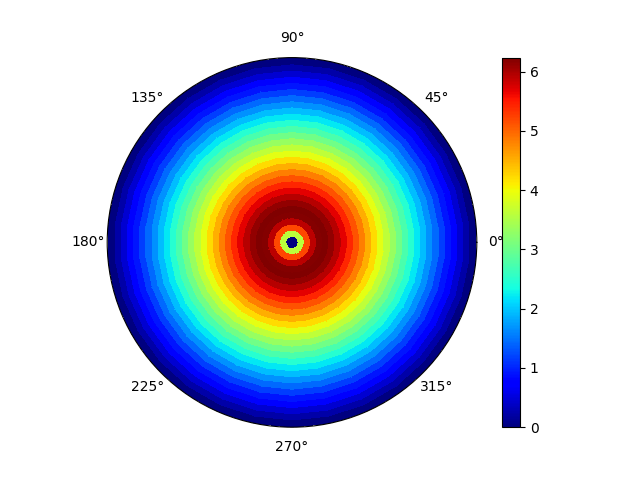
\includegraphics[scale=0.5]{test1.1.0.temperature}
\caption{Diferencia entre las temperaturas esperadas y las calculadas del test 1}
\label{fig:expected.diffs}
\end{figure}

\paragraph{} Corrimos nuestro programa teniendo en cuenta el error y confirmamos que nuestros resultados caen dentro de este rango de error aceptable. Esto se puede repetir usando el script \texttt{analyze\_expected.py}. Y muy importante es que la isoterma estimada entre ambos resultados no es muy diferente, por lo que este error no debería causar problemas. %TODO: Mejor explicación

\subsection{Revisando errores de redondeo}
\label{sec:rounding}

\paragraph{} Un problema común en la computación es que, al trabajar con números representados en una cantidad fija de dígitos binarios (bits), algo que puede ocurrir son errores de redondeo. Se busca cuantificar la diferencia entre dos tipos de representación. Para ello, queremos comparar los resultados entre usar \texttt{long double} es decir, utilizando 128-bits para guardar los números y utilizar \texttt{float} que usa 32-bits. 
\paragraph{} Armamos un sistema que genere coeficientes "muy chiquitos" (menores que \(10^{-6}\)) y utilice temperaturas muy altas (\(T_i, T_e \geq 10^6\)). De esta manera, deberían de notarse diferencias en los resultados entre las representaciones.

\begin{figure}[H]
\centering
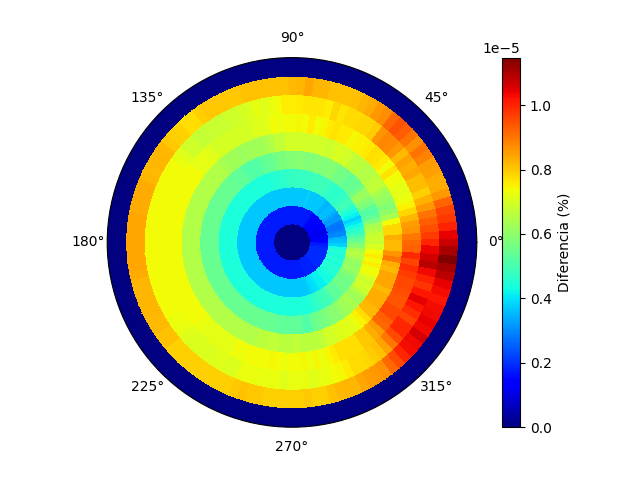
\includegraphics[scale=0.5]{rounding.temperature}
\caption{Diferencia entre las temperaturas calculadas usando \texttt{long double} y \texttt{float}}
\label{fig:rounding.diffs}
\end{figure}

\paragraph{} En la figura \ref{fig:rounding.diffs} se pueden ver las diferencias causadas. Parte de estos errores se deben a lo mencionado en la sección \ref{sec:expected} ya que los algoritmos propuestos tienen un leve error de redondeo. Observemos que los errores crecen hacia el centro del horno, esto sucede por cómo se resuelve el sistema, ya que los resultados de las temperaturas más externas se usan para calcular las más internas, por lo que el error se acumula hacia el centro. Y no hay error en las temperaturas del radio interno y del radio externo, porque estos son datos de entrada y no calculados.

\paragraph{} Este experimento puede ser repetido modificando la entrada en \texttt{data/rounding.in} y corriendo el script \texttt{analyze\_rounding.py}.

\subsection{Movimiento de la isoterma}

\subsubsection{Movimiento de la isoterma en base a la temperatura interna}

\paragraph{} Algo interesante a estudiar, es ver cómo varía la isoterma estimada en función a la temperatura interna que medimos. Se busca comprobar que la ubicación de la isoterma esta muy relacionada a la variabilidad de la temperatura interna. Motivado por este experimento, también resaltamos puntos de fusion de los metales más trabajados en altos hornos, de esta manera se puede observar la posición de la isoterma en cada uno, los metales estudiados fueron aluminio, el cobre, el hierro, y el tungsteno \cite{big:metales}. 
\paragraph{} Para armar el experimento variamos las temperaturas internas desde 500 a 7000 grados centígrados. \\
Como se puede ver en la figura \ref{fig:isotherm_by_inner}, se observa una clara relación entre la temperatura interna del horno y la ubicación de la isoterma. %TODO: Está llegando hacia la pared %TODO pero la misma se da hasta alcanzar los 3000 grados. Aun asi, no es posible concluir que sea una clara relacion positiva, es decir, que cuanto mayor sea una mayor sera la otra, ya que luego de que la temperatura interna supera los 3300 grados la ubicacion de la isoterma termina convergiendo hasta llegar cerca de 3. 

\begin{figure}[H]
	\centering
	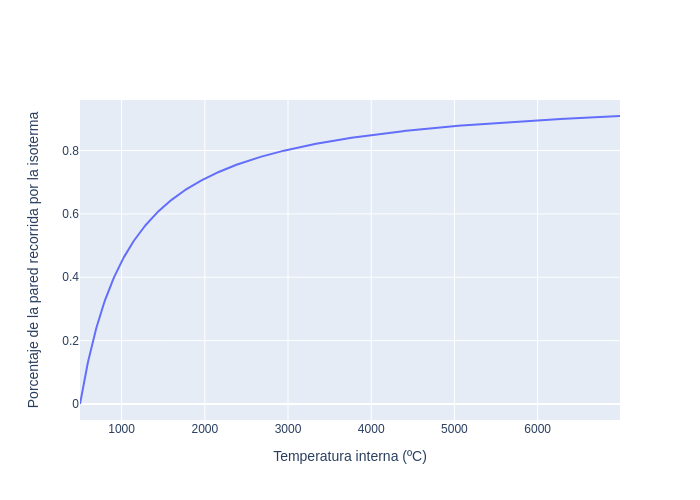
\includegraphics[scale=0.5]{isotherm_by_inner}
	\caption{Distancia de la isoterma al exterior del horno}
	\label{fig:isotherm_by_inner}
\end{figure}

Finalmente, se puede notar la ubicación de los metales elegidos aquellos que necesitan una temperatura del horno mas baja tienen la posición de su isoterma mas cercana al centro, mientras que las que requieren mas calor tienen una isoterma mas cercana a la pared exterior. 

%\subsubsection{Replicabilidad del experimento}
\paragraph{} Este experimento puede ser repetido con el script \texttt{analyze\_isotherm.py}.

\subsubsection{Movimiento de isoterma en función de la cantidad de radios}

\paragraph{} Por como se planteó la estimación de la isoterma, nos parece que la cantidad de radios dentro de la pared del horno sobre los que se trabaja afectan a la posición estimada de la isoterma. Para estudiar el efecto que tiene esta variable, analizamos los resultados cuando cambiamos la cantidad radios. Asumimos a las temperaturas internas y externas fijadas en 1500ºC y 150ºC respectivamente. \\

\begin{figure}[H]
\centering
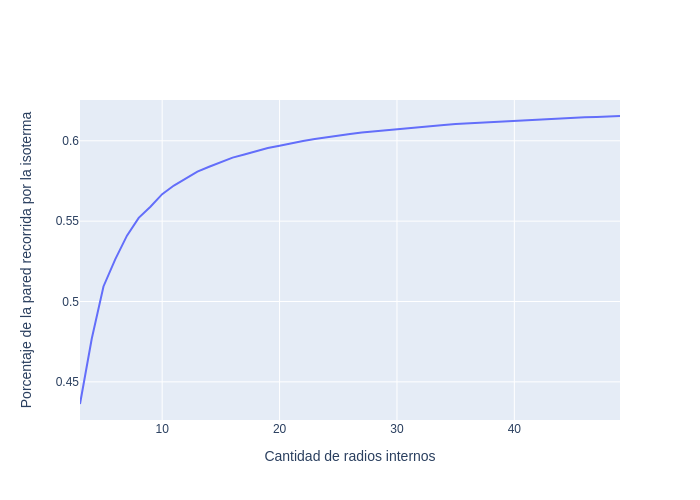
\includegraphics[scale=0.5]{isotherm_by_radii}
\caption{Posición estimada de la isoterma}
\label{fig:isotherm_by_radii}
\end{figure}

\paragraph{} Como se ve en la figura \ref{fig:isotherm_by_radii}, la posición varía bastante en base a la cantidad de radios. Preliminarmente parece convincente que si se calculan más radios se debería conseguir la estimación más correcta de la isoterma, pero habría que conseguir datos donde se sabe la posición de la isoterma, para confirmarlo.

%\subsubsection{Replicabilidad del experimento}
\paragraph{} Este experimento puede ser repetido con el script \texttt{analyze\_isotherm.py}.

\section{Conclusión}

\paragraph{} En nuestra experimentación nos encontramos con errores en los cálculos. No creemos que se deba a un error en la metodología usada, ni en la implementación. Sino a un error esperable al estar discretizando una ecuación continua, y al usar computadoras para hacer cuentas. \\
A futuro nos gustaría hacer otra implementación que aproveche diferentes técnicas de representación numérica para reducir los errores causados por la tecnología usada.
\paragraph{} Pudimos corroborar que la posición estimada de la isoterma depende de parámetros elegidos arbitrariamente. Esto resalta que las decisiones tomadas al resolver un problema pueden afectar a los resultados, y tienen que ser consideradas. 
\paragraph{} También se debería analizar la estructura material de los altos hornos, para poder definir la peligrosidad.

\pagebreak
\appendix 

\renewcommand{\thesection}{\Roman{section}}

\section{Justificación Gauss sin pivoteo} 
\label{appendix:justificacion}

\paragraph{} En este anexo demostramos que las matrices armadas (Sección \ref{sec:modelado}) son diagonal dominantes y luego justificamos inductivamente que se puede aplicar el método de Eliminación Gaussiana sin reordenar filas.

\begin{defi}
Sea \(A \in \mathbb{R}^{n \times n}\). \(A\) se dice \textbf{diagonal dominante} si 
\[
  \sum{\substack{j = 1 \\ j \neq i}}{n}|A_{ij}| \leq  |A_{ii}| \qquad \forall i = 1, ..., n
\]
\end{defi}

\begin{lema}
\label{lema:EG conserva diagonal dominante}
Sea \(A^{(0)} = A \in \mathbb{R}^{n \times n}\) una matriz diagonal dominante, con \(\sub{A}{1}{1} \neq 0\), y \(A^{(1)}\) el resultado de aplicar un paso de Eliminación Gaussiana (sin pivoteo) sobre \(A\). Entonces \(A^{(1)}\) es diagonal dominante.
\end{lema}
\begin{proof}
Consideremos la \(k\)-ésima fila de \(A^{(1)}\), queremos ver que:
\[
  \sum{\substack{k = 1 \\ k \neq i}}{n} |a^{(1)}_{i,k}| \leq |a^{(1)}_{i,i} |
\]
Se tiene que:
\[
  | a^{(1)}_{k,k} | = | a_{k,k} - \frac{a_{k,1}}{a_{1,1}} a_{1,k} |
  \qquad \text{y} \qquad
  \sum_{\substack{i = 1 \\ i \neq j}}^n | a^{(1)}_{j,i} |
= \sum_{\substack{i = 2 \\ i \neq j}}^n | a_{j,i} - \frac{a_{j,1}}{a_{1,1}} a_{1,i} |
\]
Ahora veamos como es un paso de Eliminación Gaussiana:
\[\begin{split}
  \sum_{\substack{k = 1 \\ k \neq i}}^n | a^{(1)}_{i,k} | & = \sum_{\substack{k = 2 \\ k \neq i}}^n | a_{i,k} - \frac{a_{i,1}}{a_{1,1}} a_{1,k} | \\
                                                          & \leq \sum_{\substack{k = 2 \\ k \neq i}}^n \vert a_{i,k} \vert + \left \vert \frac{a_{i,1}}{a_{1,1}} \right \vert \sum_{\substack{k = 2 \\ k \neq i}}^n \vert a_{1,i} \vert \\
                                                          & \leq \left( \vert a_{i,i} \vert - \vert a_{i,1} \vert \right) + \left \vert \frac{a_{i,1}}{a_{1,1}} \right \vert \left( \vert a_{1,1} \vert - \vert a_{1,i} \vert \right) \\
                                                          & = \vert a_{i,i} \vert - \left \vert \frac{a_{i,1}}{a_{1,1}} \right \vert \vert a_{1,i} \vert \\
                                                          & \leq \left \vert a_{i,i} -  \frac{a_{i,1}}{a_{1,1}} a_{1,i} \right \vert = | a^{(1)}_{i,i} | 
\end{split}\]
\end{proof}

\paragraph{} Ahora se tiene que luego de realizar un paso de Eliminación Gaussiana la matriz resultante también es diagonal dominante.
\paragraph{} Finalmente queda demostrar que, luego de realizar una iteración del algoritmo de Eliminación Gaussiana sin pivoteo sobre nuestra matriz, la matriz resultante queda bien definida. \\ %TODO: Definir antes que es bien definida
Entonces:
\[\begin{split}
  | a_{i,i} | & = \beta \\
              & = \left \vert - \frac{2}{(\Delta r)^2} + \frac{1}{r \Delta r} - \frac{2}{r^2 (\Delta \theta)^2} \right \vert \\
              & = \left \vert - \frac{1}{(\Delta r)^2} + \frac{1}{r \Delta r} - \frac{2}{r^2 (\Delta \theta)^2} - \frac{1}{(\Delta r)^2} \right \vert \\
              & = \left \vert - \frac{r - \Delta r}{r (\Delta r)^2} - \frac{2}{r^2 (\Delta \theta)^2} - \frac{1}{(\Delta r)^2} \right \vert \\
              & = \left \vert \frac{r - \Delta r}{r (\Delta r)^2} + \frac{2}{r^2 (\Delta \theta)^2} + \frac{1}{(\Delta r)^2} \right \vert
\end{split}\]
Veamos que si tenemos \(r_{int}, \Delta r > 0, j \geq 1\), se cumple que
\[
  r - \Delta r = (r_{int} + j \Delta r) - \Delta r = r_{int} + (j - 1) \Delta r > 0
\]
Entonces ahora sabemos que:
\[
  r - \Delta r > 0
\]
Ahora veamos como queda la sumatoria sobre una fila. Notar que:  
\[
  | \sub{a}{i}{i} | = \frac{r - \Delta r}{r (\Delta r)^2} + \frac{2}{r^2 (\Delta \theta)^2} + \frac{1}{(\Delta r)^2}
\]
Ahora al sumar los módulos del resto de los coeficientes queda que:
\[\begin{split}
  \psum{\substack{k = 1 \\ k \neq i}}{(m+1)n} |\sub{a}{i}{k}^{j}| & = |\alpha| + |\gamma| + 2 |\chi| \\
                                                                  & = \left \vert \frac{1}{(\Delta r)^2} - \frac{1}{r \Delta r} \right \vert + 2 \left \vert \frac{1}{r^2 (\Delta \theta)^2} \right \vert + \left \vert \frac{1}{(\Delta r)^2} \right \vert \\
                                                                       & = \left \vert \frac{r - \Delta r}{r (\Delta r)^2} \right \vert + \frac{2}{r^2 (\Delta \theta)^2} + \frac{1}{(\Delta r)^2} \\
                                                                       \text{(Por lo probado antes)}
                                                                       & = \frac{r - \Delta r}{r (\Delta r)^2} + \frac{2}{r^2 (\Delta \theta)^2} + \frac{1}{(\Delta r)^2} \\
                                                                       & = | \sub{a}{i}{i} |
\end{split}\] %TODO: Era \proof?

\paragraph{} Así de la demostración anterior se obtuvo que la matriz \(A \in \mathbb{R}^{(m+1)n \times (m+1)n}\) de nuestro sistema es diagonal dominante y aparte no tiene ceros en la diagonal. Ahora resta ver que la Eliminación Gaussiana es aplicable y se puede utilizar sin pivoteo. Así solamente hay que ver que para los puntos del medio del horno puede aplicarse Eliminación Gaussiana y ademas la matriz resultante es diagonal dominante. 

\begin{itemize}
\item En las primeras y últimas \(n\) filas, la matriz ya está triangulada, por lo que no hace falta aplicar Gauss.

\item[\textbf{Caso base:}] Notemos que \(\sub{a}{1}{1} = 1\) no es nulo, entonces se puede aplicar el primer paso de la Eliminación Gaussiana. Dado que \(\sub{a}{1}{2} =0\) entonces si aplicamos un paso de Eliminación Gaussianaen en el lugar $a_{2,2}$ queda un coeficiente no nulo y dado que la matriz luego de haber procesado la primer fila sigue siendo diagonal dominante entonces puedo aplicar el siguiente paso de Eliminación Gaussiana. %TODO: Revisar

\item[\textbf{HI:}] Tomamos como Hipótesis Inductiva que la matriz \(A^{(k-1)}\), obtenida tras aplicar \(k-1\) pasos de Eliminación Gaussiana sobre \(A\), es diagonal dominante y su \(k\)-ésima fila es no nula. Esto implica que \(\sub{a^{(k-1)}}{k}{k} \neq 0\).

\item[\textbf{Paso inductivo:}] Vamos a escribir a \(A^{(k-1)}\) por bloques de la siguiente manera:
\[
  A^{(k-1)} = \Gpmatrix{
    \sub{A^{(k-1)}}{1}{1} & B \\
    C & \sub{A^{(k-1)}}{2}{2} \\
  }
\]
Con \(\sub{A^{(k-1)}}{1}{1} \in \mathbb{R}^{(k-1) \times (k-1)}\). \\ %TODO: Y el resto?
%Con \(\sub{A^{(k-1)}}{1}{1} \in \mathbb{R}^{(k-1) \times (k-1)}, B \in \mathbb{R}^{(m+1)n \times (m+1)n - (k-1)}, C \in \mathbb{R}^{(m+1)n - (k-1) \times (k-1)}, \sub{A^{(k-1)}}{2}{2} \in \mathbb{R}^{(m+1)n - (k-1) \times (m+1)n - (k-1)}\). \\ %TODO: Formatting
Luego de haber probado lo anterior, sabemos que \(\sub{A^{(k-1)}}{1}{1}\) y \(\sub{A^{(k-1)}}{2}{2}\) son matrices diagonal dominantes. \\
Como para armar \(A^{(k-1)}\) ya aplicamos \((k-1)\) pasos de la Eliminación Gaussiana, se tiene que \(C = 0\). \\
Entonces cuando se quiere aplicar un paso de Eliminación Gaussiana sobre \(\sub{A^{(k-1)}}{2}{2}\), dado que el elemento de la diagonal es no nulo, este paso se puede hacer sin pivotear la matriz, y utilizando el lema \ref{lema:EG conserva diagonal dominante} se sigue que la matriz luego de este paso sera diagonal dominante.

%En caso de que la fila corresponda a un punto en la pared interna del horno, entonces esa ecuacion esta igualada a 0, para ciertos $j = 1, \dots, m - 1$ y $k = 0, \dots, n - 1$. Puntualmente, por la forma en la que se construye la matriz del sistema, el elemento $a_{u+1,u+1+n}$ es el coeficiente de la variable $t_{j,k+1}$ en dicha ecuación, que es necesariamente no nulo. Por otra parte, como la matriz $\mat{A}$ es \emph{banda} $n, n$, todos los elementos de la columna $u+1$ que se encuentran por encima de $a_{u+1,u+1+n}$ deben ser nulos. Esto quiere decir que ninguna de las iteraciones ya ejecutadas de Eliminación Gaussiana modificaron este coeficiente, y por lo tanto, sigue siendo no nulo.

\paragraph{} Solo resta probar que la fila \(k+1\) de la matriz \(A^{(k)}\) es no nula. \\
Si la fila $k$ corresponde a uno de los puntos extremos de la pared del horno, es decir, si \(1 \leq k \leq n \text{ ó } mn \leq k \leq (m+1)n\), tendrá un $1$ en la diagonal y $0$ en las demás posiciones, entonces no cambia en ningún paso de la Eliminación Gaussiana. \\
Pero si la fila corresponde a una de los puntos internos de la pared, entonces ya que cada fila representa a una instancia de la ecuación de Laplace, se tiene que el elemento \(\sub{a}{k+1}{k+1+n-1}\) es el coeficiente de la temperatura \(\sub{t}{j}{k+1}\) que es no nulo. %TODO: Lo de las columnas no es cierto

%Si la fila representa a un coeficiente de la ecuación de calor, para ciertos $j = 1, ..., m - 1$ y $k = 0, ..., n - 1$. Puntualmente, por la forma en la que se construye la matriz del sistema, el elemento $a_{k+1,k+1+n-1}$ es el coeficiente de la temperatura $t_{j,k+1}$ en dicha ecuación, debe ser no nulo. Dado como esta armado el sistema todos los elementos de la columna $k+1$ que se encuentran por arriba de $a_{k+1,k+1+n-1}$, deben ser nulos, es decir, en una iteracion de gauss no deberían haberse modificado el coeficiente $a_{k+1,k+1+n-1}$ entonces sigue siendo no nulo.
\end{itemize}

\section{Efectividad de la factorización LU}

\paragraph{} Para resolver un sistema de ecuaciones cualquiera planteado como \(Ax = b\), se puede usar el método de Eliminación Gaussiana o "Gauss", que tiene un tiempo de operación en el orden de \(\bigO{n^3}\). Pero también se puede resolver usando la factorización LU, que son dos matrices tales que \(A = LU\), donde \(L\) es triangular inferior y \(U\) es triangular superior. La forma de resolverlo así sería primero calcular un \(y\) tal que \(Ly = b\) y luego resolver \(Ux = y\). Esto toma \(\bigO{n^2}\) operaciones.
\paragraph{} Como vimos en el apéndice \ref{appendix:justificacion}, se puede aplicar Gauss sobre la matriz de nuestro sistema. Lo cual es condición suficiente para afirmar que tiene factorización \(A = LU\) \cite{clases}. Que nos es muy útil cuando queremos resolver múltiples instancias de \(At_i = b_i\) ya que la factorización LU se puede calcular aplicando la Eliminación Gaussiana una sola vez con, y resolver cada instancia \(LUt_i = b_i\) requiere muchas menos operaciones. \\
En la figura \ref{fig:solve.time} se puede confirmar que resolver una instancia del sistema con LU es definitivamente más rápido que resolverla con Gauss. 

\begin{figure}[H]
\centering
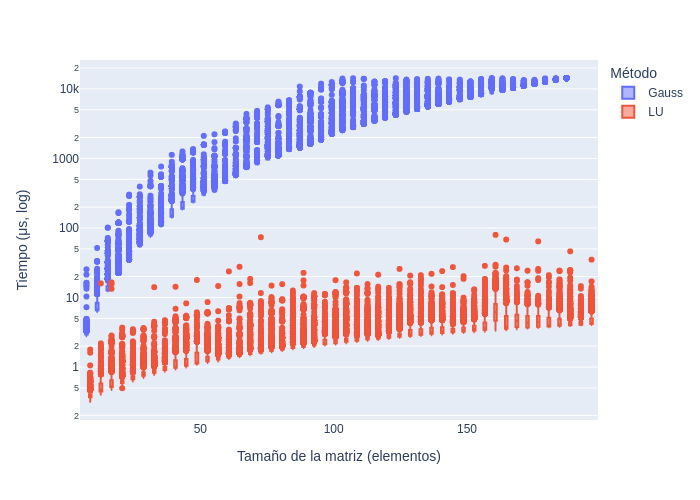
\includegraphics[scale=0.5]{times.1.t_solve}
\caption{Tiempo para resolver una instancia del sistema (1000 reps)}
\label{fig:solve.time}
\end{figure}

\begin{figure}[H]
\centering
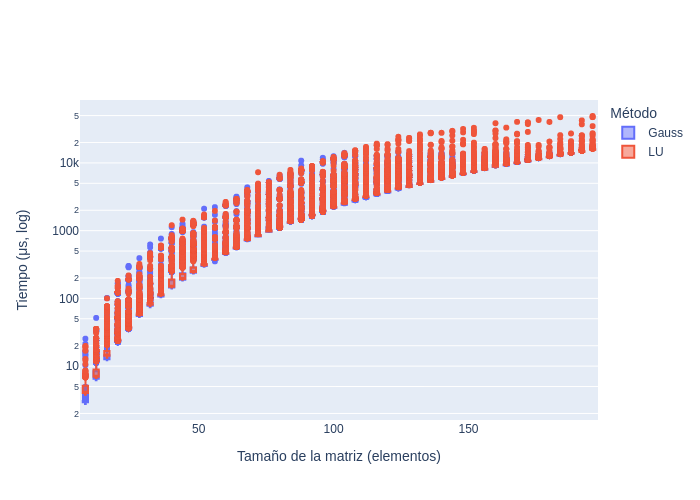
\includegraphics[scale=0.5]{times.1.t_solve_lu}
\caption{Tiempo para resolver un sistema contando el tiempo para calcular \(LU\) (1000 reps)}
\label{fig:solve.lu.time}
\end{figure}

\paragraph{} Pero como mencionamos, para calcular la factorización hay que aplicar Gauss una vez, por lo que en realidad nos queda el resultado de la figura \ref{fig:solve.lu.time} para resolver una instancia. \\
Es por esto que es importante revisar cuándo de verdad nos empieza a convenir usar la factorización \(LU\). En la figura \ref{fig:pct_lu.time} se ve que independiente del tamaño de la matriz, el tiempo usado para resolver una instancia del sistema es una fracción mínima del tiempo usado para calcular la factorización. Por lo que para dos o más instancias del sistema conviene calcular y usar la factorización \(LU\) (resaltado en la figura \ref{fig:time.2solve}). \\
En la figura \ref{fig:time.9solve} resaltamos que para resolver 9 instancias del sistema la diferencia de tiempo ya se vuelve muy notoria.

\begin{figure}[H]
\centering
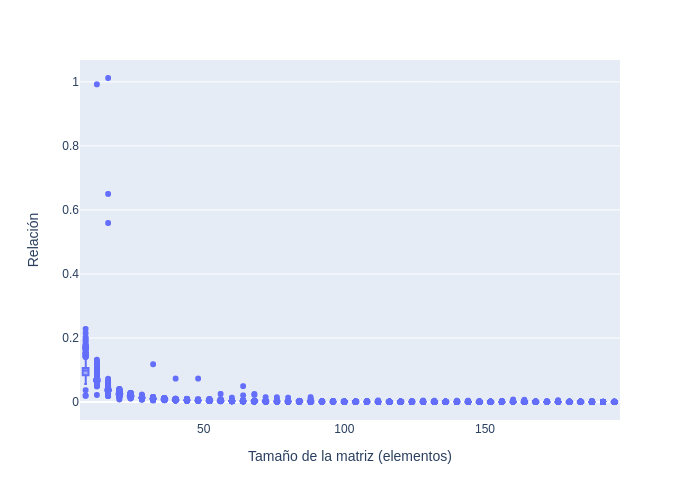
\includegraphics[scale=0.5]{times.1.t_pct_lu}
\caption{Relación entre el tiempo para resolver el sistema y el tiempo para calcular la factorización LU (1000 reps)}
\label{fig:pct_lu.time}
\end{figure}

\begin{figure}[H]
\centering
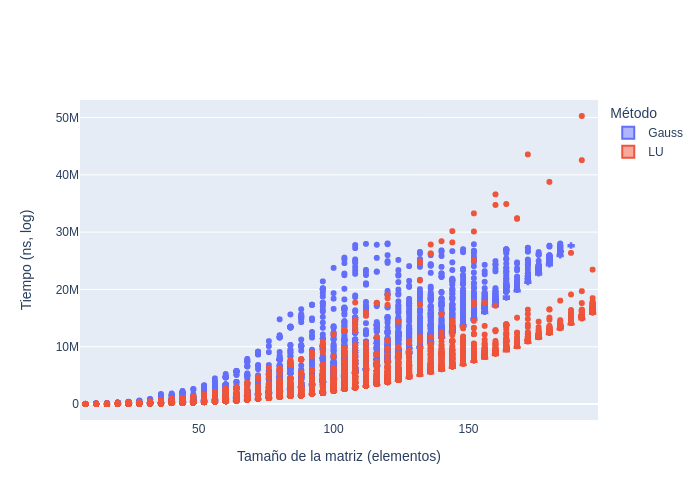
\includegraphics[scale=0.5]{times.2.t_solve_lu}
\caption{Tiempo para resolver dos instancias del sistema teniendo en cuenta el tiempo de \(LU\) (1000 reps)}
\label{fig:time.2solve}
\end{figure}

\begin{figure}[H]
\centering
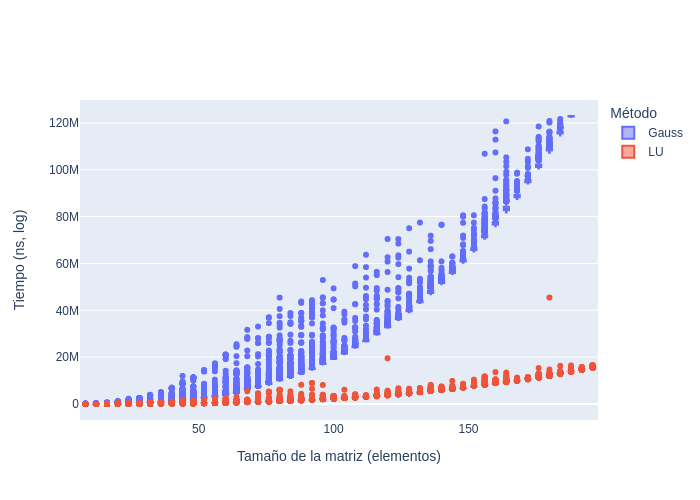
\includegraphics[scale=0.5]{times.9.t_solve_lu}
\caption{Tiempo para resolver nueve instancias del sistema teniendo en cuenta el tiempo de \(LU\) (1000 reps)}
\label{fig:time.9solve}
\end{figure}

\pagebreak
\listoffigures

\begin{thebibliography}{9}
\bibitem{how.it.works}
American Iron and Steel Institute (2005). %\href{https://web.archive.org/web/20070510164459/http://www.steel.org/AM/Template.cfm?Section=Home&template=%2FCM%2FHTMLDisplay.cfm&ContentID=5433}{How A Blast Furnace Works}. steel.org

\bibitem{clases}
R. Burden y J.D.Faires, Análisis numérico, International Thomson Editors, 2002.

\bibitem{big:metales}
Temperatura de fusión de metales. \url{https://www.redproteger.com.ar/temp_fusion.htm}

\end{thebibliography}

\end{document}

%TODO: Math formatting
